\begin{itemize}
	\item
 \end{itemize}
\subsection{Polynomial Regression}
\paragraph{Definition}
Historically when the relationship between the response and the
predictors is non-linear we used to replace the standard linear model
$$
y_{i}=\beta_{0}+\beta_{1}x_{i}+\epsilon_{i}
$$
with a polynomial function:
\begin{center}
\enc{$
y_{i}=\su{{r=0}}{d}\beta_{r}x_{i}^{r}
$}
\end{center}
Generally speaking, \tB{it is unusual to use $d$ greater than 3 or 4}.

\begin{python}
import pandas as pd
import sklearn
from sklearn.preprocessing import PolynomialFeatures
from sklearn.linear_model import LinearRegression
from sklearn.pipeline import Pipeline

df = pd.read_csv('myFile.csv', sep=';')
y, X = df.iloc[:, 0].values, df.iloc[:, 1].values.reshape(-1, 1)

model = Pipeline([
  ('poly', PolynomialFeatures(degree=3)),
  ('linear', LinearRegression(fit_intercept=False))
  ])
model = model.fit(X, y)
print(model.score(X, y))
\end{python}

\subsection{Step functions}
\begin{itemize}
	\item
 \end{itemize}

\subsection{Basis functions}
\begin{itemize}
 \item
 \end{itemize}

\subsection{Regression splines}
\paragraph{Piecewise Polynomials}
\tB{It involves fitting separate low-degree polynomials over different 
regions of $X$.}\\
The points where the coefficients change are called \tR{\emph{knots}}.
It is a function $f(X)$ that is obtained by dividing the domain of $X$ into contiguous intervals,
and representing $f$ by a separate polynomial in each interval.
More generally, an order$-M$ spline with knots $\zeta_{j}, j\in\inter{1}{K}$ is a 
piecewise-polynomial of order $M$, and has continuous derivatives up to order $M-2$.
Likewise the general form for the truncated-power basis set would be:
\begin{align*}
h_{j}(X) &= X^{j-1}, &j\in\inter{1}{M}\\
h_{M+j} &=\left(X-\zeta_{l}\right)_{+}^{M-1}, &l\in\inter{1}{K}
\end{align*}

%\paragraph{Constraints and Splines}
%We can fit a piecewise polynomial under the constraint that the fitted
%curve must be continuous.

\paragraph{The spline Basis Representation}
A cubic spline with $K$ knots can be modeled as:
\begin{center}
\enc{$
y_{i}=\beta_{0}+\su{{r=1}}{K+3}\beta_{r}b_{r}(x_{i})
$}
\end{center}
for an appropriate choice of \emph{basis functions} $\prth{b}{i}{K+3}$\\
The most direct way to represent cubic spline is \tB{to start off with
a basis for a cubic polynomial -namely, $x, x^{2}, x^{3}$ -and then add
one \emph{truncated power basis} function per knot}.
A truncated power basis function, for a cubic polynomial, is defined as:
\begin{center}
\enc{$
h(x,\zeta) = (x-\zeta)_{+}^{3}=
\left\{
\begin{array}{ll}
	(x-\zeta)^{3}&\mbox{if }x>\zeta\\
	0&\mbox{otherwise}
\end{array}
\right.
$}
\end{center}
where $\zeta$ is the knot.\\
In order to fit a cubic spline to a data set with $K$ knots, we perform
least squares regression with an intercept and $3+K$ predictors of the
form $X, X^{2}, X^{3}, h\left(X,\zeta_{1}\right), h\left(X,\zeta_{2}\right),,..,h\left(X,\zeta_{K}\right)$ where $\prth{\zeta}{i}{K}$ are the
knots. This amounts to estimating a total of $K+4$ regression 
coefficients.\\
Cubic splines are popular because most human eyes cannot detect 
discontinuity at the knots.

\begin{figure}[H]
	\begin{center}
		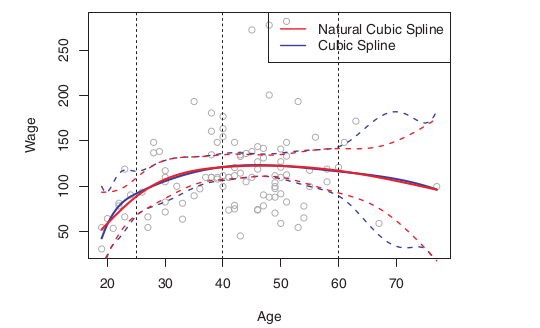
\includegraphics[width=.7\textwidth]{./chap/1chap/6sec/images/1splines.png}
	\end{center}
	\caption{A cubic spline and a natural cubic spline, with 3 
	knots, fit to a subset of the Wage data, confidence interval as
	dashed lines.}
	\label{fig:6.1splines}
\end{figure}
A natural spline is a regression spline with additional boundary 
constraints: the function is required to be linear at the boundary (in
the region where $X$ is smaller than the smallest knot, or larger than
the largest knot).\\
\tB{This frees up $4$ degrees of freedom ($2$ constraints each in both boundary regions), which
can be spent more profitably by sprinkling more knots in the interior region. }
A natural cubic spline with $K$ knots is represented by $K$ basis functions.
\begin{center}
	$\begin{cases}
		N_{1}(X) = 1\\
		N_{2}(X) = X
	\end{cases}
	,~ N_{k+2}(X) = d_{k}(X)-d_{K-1}(X)$
\end{center}
where $d_{k}(X) = \dfrac{\left(X-\zeta_{k}\right)_{+}^{3} - \left(X-\zeta_{K}\right)_{+}^{3}}{
\zeta_{K}-\zeta_{k}}$

\paragraph{Choosing the Number and Locations of the Knots}
One option is \tB{to place more knots in places where we feel the 
function might vary most rapidly}, and to place fewer knots where it 
seems more stable.\\
\sR{For the number of knots we can use cross-validation.}

\begin{python}
import pandas 
import statsmodels.api as sm
import sklearn
from sklearn.model_selection import KFold
import patsy
from patsy import dmatrix

# Choosing the good number of knots
y, x = df.iloc[:, 0], df.iloc[:, 1]
kf = KFold(n_splits=5)
n = 52
cv_set = {str(i):0 for i in range(1, n)}
for i in range(1, n):
    n_knots = i
    knot_list = np.quantile(x, np.linspace(0, 1, n_knots + 2))[1:-1]
    mse_list = []
    for train, test in kf.split(x):
        x_natural = dmatrix('cr(x, knots=knot_list)', {'x':x[train]})
        fit_natural = sm.GLM(y[train], x_natural).fit()
        yhat = fit_natural.predict(dmatrix('cr(x, knots=knot_list)', {'x':x[test]}))
        mse = ((yhat-y[test])**2).mean()
        # mse_list.append(mse)
        mse_list.append(mse)
        # print(mse)
    cv_set[str(i)] = np.array(mse_list).mean()
cv_list = list({k:v for k,v in sorted(cv_set.items(), key=lambda item: item[1])})


n_knots = int(cv_list[0])
knot_list = np.quantile(x, np.linspace(0, 1, n_knots + 2))[1:-1]
# Natural
x_natural = dmatrix('cr(x, knots = knot_list)', {'x':x})
fit_natural = sm.GLM(y, x_natural).fit()

# Create spline
xp = np.linspace(x.min(), x.max(), 50)
line_natural = fit_natural.predict(dmatrix('cr(xp,knots=knot_list)',
                                           {'xp':xp}))

plt.figure()
plt.scatter(df.iloc[:, 0], df.iloc[:, 1])
plt.plot(xp, line_natural, color='red', label="Natural Spline Regression")
for k in knot_list:
    plt.axvline(k, color='gray', ls='--')
plt.legend()
plt.show()
\end{python}
\paragraph{Comparison to Polynomial Regression}
Regression splines give superior results to polynomial regression.\\
\sB{This is because unlike polynomials, which must use a higher degree 
to produce flexible fits, splines introduce flexibility by increasing
the number of knots but keeping the degree fixed.}\\
Splines produce also more stable estimates.

\subsection{Smoothing splines}
\begin{itemize}
	\item
 \end{itemize}

\subsection{Local regression}
\paragraph{Span}
It plays a role like that of the tuning parameter $\lambda$ in 
smoothing splines: \tB{it controls the flexibility of the non-linear fit}.\\
\sT{The smaller the value of $s$, the more \emph{local} will be our fit.}

\paragraph{Algorithm: \emph{Local Regression} at $X=x_{0}$}
\begin{figure}[H]
	\begin{center}
		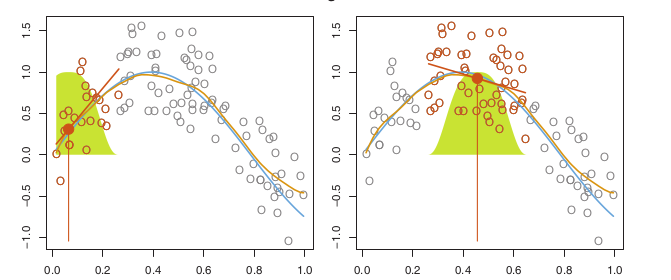
\includegraphics[width=\textwidth]{./chap/1chap/6sec/images/2localRegression.png}
	\end{center}
	\caption{Blue curve represents $f(x)$ from which the data were
	generated.\\
	Orange curve corresponds to the local regression estimate $f(x)$.\\
	Orange colored points are local to the target point $x_{0}$.\\
	Yellow-bell-shape superimposed on the plot indicates weights 
	assigned to each point, decreasing to zero with distance from
	the target point.}
	\label{fig:6.1localRegression}
\end{figure}
\begin{enumerate}
	\item Gather the fraction $s=\frac{k}{n}$ of training points
		whose $x_{i}$ are closet to $x_{0}$
	\item Assign a weight $k_{i0}=K(x_{i},x_{0})$ so that \tB{the
		point furthest from $x_{0}$ has weight zero, and the 
		closet has the highest weight}.\\
		\sB{All but these $k$ nearest neighbors get weight 0}
	\item \tB{Fit a weighted least squares regression of the $y_{i}
		$ on the $x_{i}$}, using the aforementioned weights, by
		\tB{finding $\beta_{0}$ and $\beta_{1}$ that minimize:
		$$\su{{i=1}}{n}K_{i0}(y_{i}-\beta_{0}-\beta_{1}x_{i})^{2}$$}
	\item \tB{The fitted value at $x_{0}$ is given by $\hat{f}(x_{
		0})= \hat{\beta}_{0}+\hat{\beta}_{1}x_{0}$}
\end{enumerate}
For $p$-dimensional neighborhoods, local regression can perform poorly
if $p$ is much larger than 3 or 4, because there will generally be very
few training observations close to $x_{0}$

\subsection{Generalized additive models}
\emph{Generalized Additive Models} (GAMs) \sB{provide a genral 
framework for extending a standard linear model by allowing non-linear}
functions of each of the varialbes, \sB{while maintaining additivity}.

\paragraph{Principle}
\subparagraph{Definition}
Considering we have $y_{i}=\beta_{0}+\su{{r=1}}{p}\beta_{r}x_{ir}+
\epsilon$\\ \tB{We replace each linear component $\beta_{j}x_{ij}$ with
a (smooth) non-linear function $f_{j}(x_{ij})$}:\\
$$
y_{i}=\beta_{0}+\su{{j=1}}{p}f_{j}(x_{ij})+\epsilon_{i}
$$
\sB{It is called an \emph{additive model} because we calculate a
separate $f_{i}$ for each $X_{j}$, and then add together all of their 
contributions.}\\
In the regression setting, a generalized additive model has the form: 
$\E{Y|\prth{X}{j}{p}}=\alpha+\su{{j=1}}{p}f_{j}(X_{j})$, the $f_{j}$'s are unspecified smooth
(``non-parametric'') functions.
\paragraph{Fitting Additive Models}
The additive model has the form:
\begin{center}
	\enc{$ Y = \alpha + \su{{j=1}}{p}f_{j}(X_{j})+\epsilon$}
\end{center}
where $\E{\epsilon}=0$. Given observations $x_{i},y_{i}$ a criterion like the penalized sum of
squares
\begin{center}
\encB{$ PRSS\left(\alpha,\prth{f}{j}{p}\right) = \su{{i=1}}{N}\left(y_{i}-\alpha-\su{{j=1}}{p}
f_{j}(x_{ij})\right)^{2} + \su{{j=1}}{p}\lambda_{j}\su{}{}f_{j}^{''}(t_{j})^{2}dt_{j}$}
\end{center}
where the $\lambda_{j}\geq 0$ are the tuning parameters.

\subparagraph{The Backfitting Algorithm for Additive Models}
\begin{enumerate}
	\item Initialize: $\forall (i,j)\in\inter{1}{N}\times\inter{1}{p}, \hat{\alpha} = \dfrac{1}{N}\su{{1}}{N}y_{i}, \hat{f}_{j}\equiv 0$
	\item Cycle: $j=1,\dots,p,1,\dots,p,\dots$
		\begin{align*}
			\hat{f}_{j} &\leftarrow \bm{S}_{j}\left[\left\{y_{i}-\hat{\alpha}-
			\su{{k\neq}}{}\hat{f}_{k}(x_{ik})\right\}_{1}^{N}\right]\\
			\hat{f}_{j} &\leftarrow \hat{f}_{j}-\dfrac{1}{N}\su{{i=1}}{N}\hat{f}_{j}(x_{ij})
		\end{align*}
		until the function $\hat{f}_{j}$ change less than a pre-specified threshold.
\end{enumerate}
We set \sB{$\hat{\alpha}=ave(y_{i})$} and it never changes. We apply a \sB{cubic smoothing spline  
$S_{j}$} to the targets $\left\{y_{i}-\hat{\alpha}-\su{{k\neq j}}{}\hat{f}_{k}(x_{ik})\right\}_{1}^{N
}$. The process is continued unitil the estimates $\hat{f_{j}}$ stabilize.\\ \sB{The backfitting 
procedure allow one to choose a fitting method appropriate for each input variable however it fits 
all predictors which is not feasible or desirable when a large number are available}

\subparagraph{Python Code}
\begin{python}
import pygam
from pygam import LinearGAM, LogisticGAM
from pygam import GAM, l, s, f, te, intercept


# REGRESSION
df_reg = pd.read_csv('myFile_reg.txt', sep=';')
y, X = df.iloc[:, 0], df.iloc[:, 1:]
p = len(X)
lgam = LinearGAM(
   eval(' + '.join(['f({})'.format(i) 
       for i in range(p-3)] +
       ['l(p-3)', 'l(p-2)', 'l(p-1)'])
       )
)

lgam_grid = lgam.gridsearch(X, y)
lgam_grid.summary()

fig, ax = plt.subplots()
ax.scatter(X.budget_std, y)
ax.plot(X.budget_std, lgam_grid.predict(X), color='red')
ax.plot(X.budget_std, lgam_grid.prediction_intervals(X)[:, 0])
ax.plot(X.budget_std, lgam_grid.prediction_intervals(X)[:, 1])
plt.show()



# CLASSIFICATION
# Replace LinearGAM by LogisticGAM!!

\end{python}

\subparagraph{Pros and Cons of GAM's}
\begin{itemize}
	\item[\tV{+}] We do not need to manually try out many different
		transformations on each variable individually.
	\item[\tV{+}] The non-linear fits can potentially make more
		accurate predictions for the response $Y$
	\item[\tV{+}] Because the model is additive, we can examine the
		effect of each $X_{j}$ on $Y$ individually while 
		holding all of the other variables fixed.
		
	\item[\tV{+}] The smoothness of the function $f_{j}$ for the 
		variable $X_{j}$ can be summarized via degrees of 
		freedom.
	\item[\tR{-}] The model is restricted to be additive
\end{itemize}

\paragraph{The Naive Bayes Classifier}
It is \tB{especially appropriate when dimension $p$ of the feature space is high}, making density 
estimation unattractive. The naive Bayes model \tB{assumes that given a class $G=j$, the features
$X_{k}$ are independent}.\\
While this assumption is generally not true, it does simplify the estimation dramatically, using
class $J$ as the base we can derive:
\begin{itemize}
	\item The individual class-conditional marginal densities $f_{jk}$ can each be estimated
		separately using one-dimensional kernel density estimates.
	\item If a component $X_{j}$ of $X$ is discrete, then an appropriate histogram estimate
		can be used.
\end{itemize}

\sB{Despite these rather optimistic assumptions, naive Bayes classifiers often outperform far more
sophisticated alternatives.} Because although the individual class density estimates may be biased
this bias might not hurt the posterior probabilities as much especially near the decision regions.

\begin{align*}
	\log\left(\dfrac{\ProbC{X}{G=l}}{\ProbC{X}{G=J}}\right) =& \log\left(\dfrac{\pi_{l}f_{l}(
	X)}{\pi_{J}f_{J}(X)}\right)\\
	=& \log\dfrac{\pi_{l}\prd{{k=1}}{p}f_{lk}(X_{k})}{\pi_{J}\prd{{k=1}}{p}f_{Jk}(X_{k})}
	\text{ (independence assumption)}\\
	=& \log\left(\dfrac{\pi_{l}}{\pi_{J}}\right) + \su{{k=1}}{p}\log\left(\dfrac{f_{lk}(X_{k})}{f_{Jk}(X_{k})}\right)\\
	=& \alpha_{l} + \su{{k=1}}{p}g_{lk}(X_{k})
\end{align*}
\subparagraph{Python Code}

\begin{python}
import sklearn
from sklearn.model_selection import train_test_split
from sklearn.naive_bayes import GaussianNB

df = pd.read_csv('myFile.csv', sep=';')
y, X = df.iloc[:, 0], df.iloc[:, 1:]

X_train, X_test, y_train, y_test = train_test_split(
    X, y, test_size=0.5, random_state=0)
gnb = GaussianNB()
y_pred = gnb.fit(X_train, y_train).predict(X_test)
print('Number of mislabeled points out of a total\
%d points: %d'
% (X_test.shape[0], (y_test != y_pred).sum()))
\end{python}

\subsection{Radial Basis Functions and Kernels}
Kernel method achieve flexibility by fitting simple models in a region local to the target point
$x_{0}$. Localization is achieved via a weighting kernel $K_{\lambda}$, and individual 
observations receive weights $K_{\lambda}(x_{0}, x_{1})$.\\ 
Radial basis functions combine these ideas by treating the kernel function $K_{\lambda}(\xi, x)$.
This leads to the model:
\begin{align*}
	f(x) =& \su{{j=1}}{M}K_{\lambda}(\xi_{j},x)\beta_{j}\\
	=& \su{{j=1}}{M}D\left(\dfrac{\norm{x-\xi_{j}}}{\lambda_{j}}\right)\beta_{j}
\end{align*}
where \sB{each basis elements is indexed bya a location or \emph{prototype} parameters $\epsilon_{j}$
and a scale parameter $\lambda_{j}$}.



\subsection{Model Inference and Averaging}
\paragraph{Maximum Likelihood Inference}
The likelihood function can be used to assess the precision of $\hat{\theta}$. We need few more
definitions.
\begin{itemize}
	\item Score function: $\dot{l}(\theta,\bm{Z})=\su{{i=1}}{N}\dot{l}(\theta,z_{i}) = 
		\su{{i=1}}{N}\dfrac{\partial l(\theta;z_{i})}{\partial \theta}$ 
	\item The \emph{information matrix} is: $\bm{I}=-\dfrac{{i=1}}{N}\dfrac{\partial^{2}l(
		\theta;z_{i})}{\partial\theta\partial\theta^{T}}$
	\item \emph{Fisher information}: $\bm{i}(\theta)=\mathbb{E}_{\theta}\left(\bm{I}(\theta)\right)$
\end{itemize}

Confidence points for $\theta_{j}$ can be constructed from either approximation:
$\hat{\theta}-z^{(1-\alpha)}\sqrt{\bm{I}(\hat{\theta})_{jj}^{-1}}$
More accurate confidence intervals can be derived from the likelihood function, by using the
chi-squared approximation
$$ 2\left[l(\hat{\theta})-l(\theta_{0})\right]\hookrightarrow \chi_{p}^{2}$$
where $p$ is the number of components in $\theta$.\\
The maximum likelihood estimate is obtained by setting $\dfrac{\partial l}{\partial\beta}=
\dfrac{\partial^{2} l}{\partial\sigma^{2}}=0$ giving 
$$
\begin{cases}
	\hat{\beta} = \left(\bm{H}^{T}\bm{H}\right)^{-1}\bm{H}^{T}\bm{y}\\
	\sigma^{2} = \dfrac{1}{N}\su{}{}\left(y_{i}-\hat{\mu}(x_{i})\right)^{2}
\end{cases}
$$
The advantage of the bootstrap over the maximum of likelihood formula is that it allows us to
compute maximum likelihood estimates of standard errors and other quantities in setting where
no formulas are available.


\paragraph{The EM Algorithm}
We would like to model the density of the data points, and \sB{due to the apparent bi-modality, a
Gaussian distribution} would not be appropriate.
$
\begin{cases}
	Y_{1}\hookrightarrow\mathcal{N}(\mu_{1}, \sigma_{1}^{2})\\
	Y_{2}\hookrightarrow\mathcal{N}(\mu_{2}, \sigma_{2}^{2})\\
	Y = (1-\Delta)Y_{1} + \Delta Y_{2}
\end{cases}
$ 
where $\delta\in\left\{0,1\right\}$ with \sB{$\Prob{\Delta=1}=\pi$}\\
$$
l_{0}(\theta;\bm{Z},\bm{\Delta}) = \su{{i=1}}{N} \left[(1-\bm{\Delta}_{i})\log\left(
\phi_{\theta_{1}}(y_{i})\right) +\bm{\Delta}_{i}\log\left( \phi_{\theta_{2}}(y_{i})\right) 
\right] + \su{{i=1}}{N} \left[(1-\bm{\Delta}_{i})\log\left( 1-\pi\right) +
\bm{\Delta}_{i}\log\left(\pi\right) \right]
$$
Since the values of the $\Delta_{i}$'s are actually unknown, we proceed in an iterative fashion
substituting for each $\Delta_{i}$ in the previous equation : 
$\gamma_{i}(\theta)=\mathbb{E}_{\theta,\bm{Z}}(\Delta_{i}) = \ProbC{\theta,\bm{Z}}{\Delta_{i}=1}$
also called \sB{the \emph{responsibility}}
We use the following EM algorithm for special case of the Gaussian mixtures.
\begin{itemize}
	\item \tB{Expectation} Step: we do a soft assignment of each observation to each model:
		\sB{the current estimates of the parameters are used to assign responsibilities}
		according to the relative density of the training points under each model.
	\item \tB{Maximization} Step: These \sB{responsibilities are used in weighted 
		maximum-likelihood fits} to update the estimates of the parameters.
\end{itemize}
The EM algorithm is a popular tool for simplifying difficult maximum likelihood problems.
\subparagraph{EM Algorithm for 2-Component Gaussian Mixture}
\begin{enumerate}
	\item  Take initial guesses for the parameters $\hat{\mu}_{1}, \hat{\sigma}_{1}, \hat{\mu}_{2}, \hat{\sigma}_{2}, \hat{\pi}$
	\item Excpectation Step: compute the responsibilities: 
		$\hat{\gamma}_{i}=\dfrac{\hat{\pi}\phi_{\hat{\theta}_{2}}(y_{i})}{(1-\hat{\pi})\phi_{\hat{\theta}_{1}}(y_{i}) + \hat{\pi}\phi_{\hat{\theta}_{2}}(y_{i})}$ for $i\inter{1}{N}$
	\item Maximization Step: compute the weighted means and variances
		\begin{align*}
			\hat{\mu}_{1} = \dfrac{\su{{i=1}}{N}(1-\hat{\gamma}_{i})y_{i}}{\su{{i=1}}{N}(1-\hat{\gamma}_{i})}&, & 
			\hat{\sigma}_{1} = \dfrac{\su{{i=1}}{N}(1-\hat{\gamma}_{i})(y_{i}-\hat{\mu}_{1})^{2}}{\su{{i=1}}{N}(1-\hat{\gamma}_{i})}\\
			\hat{\mu}_{2} = \dfrac{\su{{i=1}}{N}\hat{\gamma}_{i}y_{i}}{\su{{i=1}}{N}\hat{\gamma}_{i}}&, & 
			\hat{\sigma}_{2} = \dfrac{\su{{i=1}}{N}\hat{\gamma}_{i}(y_{i}-\hat{\mu}_{2})^{2}}{\su{{i=1}}{N}\hat{\gamma}_{i}}
		\end{align*}
	\item Iterate steps 2 and 3 until convergence
\end{enumerate}
and the mixing probability $\hat{\pi}=\su{{i=1}}{N}\dfrac{\hat{\gamma}_{i}}{N}$

\begin{python}
import sklearn
from sklearn.mixture import GaussianMixture

df = pd.read_csv('myFile.csv', sep=';')
y, X = df.iloc[:, 0], df.iloc[:, 1:]

model = GaussianMixture(n_components=2,
    init_params='random')
model.fit()
y_pred = model.predict(X)
\end{python}

\paragraph{The EM Algorithm in General}
Our observed data is $\bm{Z}$ having log-likelihood $l(\theta,\bm{Z})$. The latent or missing data
is $\bm{Z}^{m}$, so that the complete data is $\bm{T}=(\bm{Z},\bm{Z}^{m})$ with log-likelihood 
$l_{0}(\theta,\bm{T})$. In the mixture problem $(\bm{Z},\bm{Z}^{m}) = (\bm{y},\bm{\Delta})$
Since $\ProbC{\bm{Z},\theta'}{\bm{Z}^{m}}=\dfrac{\ProbC{\theta'}{\bm{Z}^{m},\bm{Z}}}{\ProbC{\theta'}{\bm{Z}}}$ we can write:
$\ProbC{\theta'}{\bm{Z}}=\dfrac{\ProbC{\theta'}{\bm{T}}}{\ProbC{\bm{Z},\theta'}{\bm{Z}^{m}}}$.
In terms of log-likelihoods, we have:
$$ l(\theta';\bm{Z}) = l_{0}(\theta'; \bm{T}) - l_{1}(\theta';\bm{Z}^{m}|bm{Z})$$ where $l_{1}$ is
based on the conditional density: $\ProbC{\bm{Z},\theta'}{\bm{Z}^{m}}$
\begin{enumerate}
	\item Start with initial guesses for the parameters $\hat{\theta}^{(0)}$
	\item Expectation Step: at the $j^{th}$ step, compute 
		$$ Q(\theta',\hat{\theta}^{(j)}) = \E{l_{0}(\theta':\bm{T})|\bm{Z},\hat{
		\theta}^{j)}}$$
	\item Maximization Step: determine the new estimate $\hat{\theta}^{(j+1)}$ as the 
		maximizer of $Q\left(\theta',\hat{\theta}^{(j)}\right)$ over $\theta'$
	\item Iterate steps 2 and 3 until convergence
\end{enumerate}
In the M step, the EM algorithm maximizes $Q(\theta', \theta)$ over $\theta'$ rather than
actual objective function $l(\theta':\bm{Z})$
\subparagraph{EM as a Maximization Procedure}
Here is a different view of the EM procedure, as a joint maximization algorithm. Consider 
function:
$$ F(\theta',\tilde{P})= \mathbb{E}_{\tilde{P}}\left(l_{0}(\theta':\bm{T})\right)-
\mathbb{E}_{\tilde{P}}\left(\tilde{P}(\bm{Z}^{m})\right)$$
Here $\tilde{P}(\bm{Z}^{m})$ is any distribution over the latent data $\bm{Z}^{m}$

The  function $F$ expands the domain of the log-likelihood, to facilitate its maximization.
The maximizer over $$\tilde{P}(\bm{Z})=\ProbC{\bm{Z},\theta'}{\bm{Z}}$$
\begin{figure}[H]
	\begin{center}
		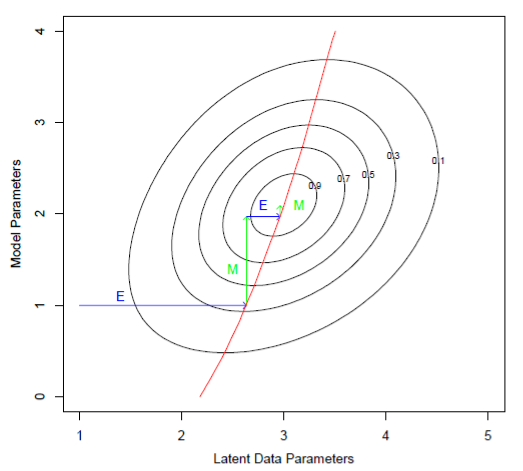
\includegraphics[width=.5\textwidth]{./chap/1chap/6sec/images/3_emAlgo.PNG}
	\end{center}
	\caption{The contours of the (augmented) observed data log-likelihood $F(\theta,\tilde{P})$
	The $E$ step is equivalent to maximizing the log-likelihood over the parameters of the 
	latent data distribution. The $M$ step maximizes it over the parameters of the 
	log-likelihood. The red curve corresponds to the observed data log-likelihood a profile
	obtained by maximizing $F(\theta', \tilde{P})$ for each value of $\theta'$}
	\label{fig:3_emAlgo}
\end{figure}
\subparagraph{Gibbs Sampler}
\begin{enumerate}
	\item Take some initial values $U_{k}^{(0)}$ for $k\in\inter{1}{K}$
	\item Repeat for $t\in\inter{1}{?}$:
		For $k\in\inter{1}{K}$ generate $U_{k}^{(t)}$ from 
		$$ \Pr(U_{k}^{(t)}|U_{1}^{(t)}, \cdots U_{k-1}^{(t)}, U_{k+1}^{(t-1)},\cdots U_{K}^{(t-1)})$$
	\item Continue step 2 until the joint distribution of $\left( U_{j}^{(t)} \right)_{1\leq j\leq K}$
\end{enumerate}
\paragraph{MCMC (Markov chain Monte Carlo) for Sampling from the Posterior}
Gibbs sampling  is an MCMC procedure that is closely related to the EM Algorithm: the main 
difference  is that is it samples from the conditional distributions rather than maximizing over 
them. \\
More formally, Gibbs sampling produces a Markov chain whose stationary distribution is the 
true joint distribution, and hence the term of ``Markov Chain Monte Carlo''
\subparagraph{Gibbs sampling for mixtures}
\begin{enumerate}
	\item Take some initial values: $\theta^{(0)}=(\mu_{1}^{(0)}, \mu_{2}^{(0)})$
	\item Repeat for $t\in\inter{1}{?}$:
		\begin{enumerate}[label=(\alph*)]
			\item For $i\in\inter{1}{N}$ generate $\bm{\Delta}_{i}^{(t)}\in\left\{0,1
				\right\}$ with $\Prob{\bm{\Delta}_{i}^{(t)}=1}=\hat{\gamma}_{i}(
				\theta^{(t)})$
			\item Set
				\begin{align*}
					\hat{\mu}_{1} = & \dfrac{\su{{i=1}}{N}\left(1-\bm{\Delta}_{i}^{(t)}\right)y_{i}}{\su{{i=1}}{N}\left(1-\bm{\Delta}_{i}^{(t)}\right)}\\
					\hat{\mu}_{2} = & \dfrac{\su{{i=1}}{N}\bm{\Delta}_{i}^{(t)}y_{i}}{\su{{i=1}}{N}\bm{\Delta}_{i}^{(t)}}
				\end{align*}
					and generate $\mu_{1}^{(t)}\hookrightarrow\mathcal{N}(\hat{\mu}_{1}, \hat{\sigma}_{1}^{2})$ and $\mu_{1}^{(t)}\hookrightarrow\mathcal{N}(\hat{\mu}_{2},
					\hat{\sigma}_{2}^{2})$
			\item Continue until the joint distribution of $\left(\Delta^{(t)},\mu_{1}^{(t)}, \mu_{2}^{(t)}\right)$ does not change.
		\end{enumerate}
\end{enumerate}

\paragraph{Bagging}
We show how to use the bootstrap to improve the estimate or prediction itself.\\
For each bootstrap $\bm{Z}^{*b}$ for $b\in\inter{1}{B}$ we fit our model, giving prediction
$\hat{f}^{*b}(x)$. The bagging estimate is defined by:
$$ \hat{f}_{bag}(x) = \dfrac{1}{B}\su{{b=1}}{B}\hat{f}^{*b}(x)$$
It is a Monte Carlo estimate of the true bagging estimate, approaching it as $B\rightarrow \infty$.o
Suppose $\xi$
\paragraph{Model Averaging and Stacking}
The posterior distribution of $\xi$ is
$$ \ProbC{\bm{Z}}{\xi} = \su{{m=1}}{M}\ProbC{M_{m},\bm{Z}}{\xi}\ProbC{\bm{Z}}{M_{m}}$$
with posterior $\E{\xi|\bm{Z}} = \su{{m=1}}{M}\E{\xi|M_{m},\bm{Z}}\ProbC{\bm{Z}}{M_{m}}$.
This Bayesian prediction is a weighted average of the individual predictions with weights 
proportional to the posterior probability of each model. This formulation leads to a number
of different model-averaging strategies.

\paragraph{Stochastic Search: Bumping}
\emph{Bumping} uses bootstrap sampling to move randomly through model space. 
In detail we draw bootstrap samples $\left(\bm{Z}^{*j}\right)_{1\leq j\leq B}$ and fit our model
to each giving predictions $\hat{f}^{*b}(x), b\in\inter{1}{B}$. We then choose the model that 
produces the smallest prediction error, averaged over the \emph{original training set}.
$$ \hat{b}=\min\limits_{b}\su{{i=1}}{N}\left[y_{i}-\hat{f}^{*b}(x_{i})\right]^{2}$$

\subsection{lab: Non-linear modeling}
\begin{itemize}
 \item
 \end{itemize}

\subsection{Exercises}
\begin{itemize}
 \item
 \end{itemize}

